% A simple commutative diagram
% Stefan Kottwitz
\documentclass{article}
\usepackage{tikz}
\usetikzlibrary{matrix}
\begin{document}
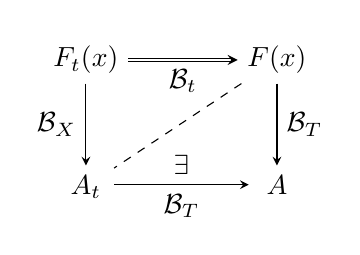
\begin{tikzpicture}
  \matrix (m) [matrix of math nodes,row sep=3em,column sep=4em,minimum width=2em]
  {
     F_t(x) & F(x) \\
     A_t & A \\};
  \path[-stealth]
    (m-1-1) edge node [left] {$\mathcal{B}_X$} (m-2-1)
            edge [double] node [below] {$\mathcal{B}_t$} (m-1-2)
    (m-2-1.east|-m-2-2) edge node [below] {$\mathcal{B}_T$}
            node [above] {$\exists$} (m-2-2)
    (m-1-2) edge node [right] {$\mathcal{B}_T$} (m-2-2)
            edge [dashed,-] (m-2-1);
\end{tikzpicture}
\end{document}
